\chapter{Probabilistic Variational Model}
\label{chap:statistical_model}

\lettrine{I}{ntroduction} into this chapter\dots

\pagebreak

\section{Time series representation and \aclp{gp}}
\label{sec:time_series_analysis}

\todo[inline]{introduction to GP. search over all functions. emphasize the aspects of it that we are using it for, but also a bit generally why it's good for ML. compare it to other interpolation/extrapolation methods. if makes sense, explain to what kind of data it suits.}

\todo[inline]{say that the novel process introduced here can be used for any dataset, and VACC is used here for demonstration}

%\subsection{Covariance functions (kernels)}
\subsection{Kernel building and tuning}
\label{subsec:covariance_functions}

\todo[inline]{current information taken from \url{http://scikit-learn.org/stable/modules/gaussian_process.html}. in the introduction add the reference(s) mention at the end of this page.}
\todo[inline]{also, there was a very detailed thesis/paper about kernels, check if there are more good details there}

Kernels (also called \textit{covariance functions} in the context of \acp{gp}) are a key component \acp{gp}, as they define the statistical relationship between the input values.
In general, they represent describe the similarity $k(x, x')$ between each pair of input points, so that $k(\cdot, \cdot)$ determines how similar the outputs $y_*$ and $y_*'$ will be. 
More formally, a covariance function can be described as $\mathcal{K}(u, v) = \phi(u) \cdot \phi(v)$, where $\phi(\cdot)$ is a function that maps the input vectors into a transformed feature space.
Which function to use is a key question when modeling using a \ac{gp}, as it determines the behavior of the model and the quality of the predictions it will be able to make.
Naturally, some assumptions and decisions regarding the data must be made when choosing a kernel.
A kernel's parameters are optimized to achieve functions that better fit the data, the consistency of the resulted functions is measured using log maximum likelihood.

Since convergence analyses usually refer to the \textit{difference} between values in different production (as opposed to the values themselves), stationary kernels are more suitable for fitting \ac{gp} to them, as they are shaped by the distances between each pair of data point rather than merely their absolute values.
%That is, they fulfill $k(x_1, x_2) = k(x_1 - x_2)$.
%This list only covers a small subset of common covariance functions.
%Further kernels include the exp-sine squared, dot-product, linear, and more.
%\putref{put 2 references about kernels, or only 1 is the first is used above}
Kernels can also be chained using multiplication or addition to combine characteristics of multiple kernels.
Multiplication-based kernels are maximized when all of its kernel factors yield high values, whereas
Addition-based kernels, are maximized when any of their addend kernels yield a high value.
%For example, multiplying a linear kernel by a periodic one will result in functions that are \textit{both} periodic \textit{and} with increasing amplitude as they move away from the origin.
For the modeling presented here, an additive kernel is used with constant, RBF, and noise terms (see \crefrange{eq:constant_kernel}{eq:RBF_kernel}).
The RBF term determines the general shape of the curve (see example in \cref{fig:RBF_prior_posterior}), the constant term enables shifting of the curve if necessary, and the noise term adds degrees of freedom in case the curve cannot completely fit the input signal.

The definitions of the individual kernels are as follows:

\begin{description}
	\item[Constant kernel -- ]
	This is a simple kernel that assigns the same value for all input pairs.
	Since by itself it does not offer a lot of characteristic to the covariance function, it is usually used as part of a product kernel, where which it scales the magnitude of the other factors, or as part of a sum kernel, in which it modifies the mean of the Gaussian process.
	It has a single parameter, the constant value, and it is defined as 
	%
	\begin{equation}
		\label{eq:constant_kernel}
		k_{constant}(C, x, x') = C\forall x_1, x_2,
	\end{equation}
	\eqname{Constant kernel}
	%
	where $C$ is the constant value parameter.
	
	\item[Noise kernel -- ]
	is a kernel used for capturing unexplained variation in the data, i.e., noise.
	It is typically based on the constant kernel as part of a sum kernel, in which it explains the noise component of a signal.
	In this context, the constant parameter is tuned to estimate the noise level.
	This is determined by
	%
	\begin{equation}
		\label{eq:noise_kernel}
		k_{noise}(\{noise\_level\}, x, x') =
		\begin{cases}
		C_{noise\_level}, & if\quad x_1 = x_2\\
		0, & otherwise,\\
		\end{cases}
	\end{equation}
	\eqname{Noise kernel}
	%
	where $noise\_level$ equals the variance of the noise found in the input signal.
	
	\item[Radial-basis function (RBF) kernel --]
	also known as \emph{squared exponential kernel}, the RBF kernel is a stationary kernel with one parameter, \emph{lengthscale} $l > 0$.
%	 which can either be a scalar (isotropic variant of the kernel) or a vector with the same number of dimensions as the inputs x (anisotropic variant of the kernel).
	This kernel typically results in generally smoothed functions, with the lengthscale being associated with the long-term smoothness and degree of variability on the time dimension.
	The RBF kernel is defined as
	%
	\begin{equation}
		\label{eq:RBF_kernel}
		k_{RBF}(\{\ell\}, x, x') = \sigma^2 exp\left(\frac{\lVert x_1 - x_2 \lVert ^2_d}{2\ell^2}\right),
	\end{equation}
	\eqname{Radial basis function (squared exponential) kernel}
	%
	where $\lVert x_1 - x_2 \lVert$ is the Euclidean distance between two $d$-dimensional input points and $\sigma^2$ is a scalar factor that determines the average distance of your function away from its mean.
	\cref{fig:RBF_prior_posterior} shows prior and posterior examples of the RBF kernel.
	
%	\item[Rational quadratic kernel]
%	This kernel can be seen as a scale mixture (infinite sum) of RBF kernels with different length scales.
%	Therefore, \acp{gp} priors with this kernel expect to see functions which vary smoothly across many length scales.
%	It has two parameters: length scale $l > 0$ and scale mixture $\alpha > 0$.
%	The parameter $\alpha$ determines the relative weighting of large-scale and small-scale variations.
%	When $\alpha$ $\lim$ $\inf$, the RQ kernel is identical to the SE kernel, as described by
%	
%	\begin{equation}
%		\label{eq:RQ_kernel}
%		k_{RQ}(\{\sigma, \alpha, \ell\}, x, x') = \sigma^2 \left( 1 + \frac{\lVert x_1 - x_2 \lVert ^2}{2\alpha \ell^2} \right)^{-\alpha}.
%	\end{equation}
%	\eqname{Rational quadratic kernel}
\end{description}

\subsection{Data interpolation using kriging}
\label{subsec:interploating_data_using_kriging}
	
\begin{figure}[t]
	\centering
	\subfigure[RBF kernel prior ($length scale = 1$)]
		{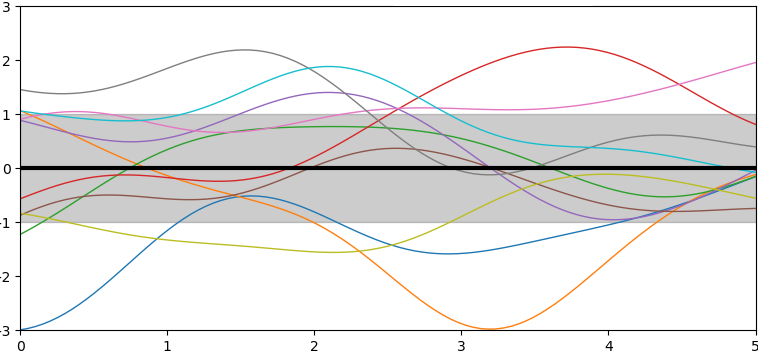
\includegraphics[width=0.45\textwidth]{RBF_prior}
	\label{fig:RBF_prior}}
	\hfill % no empty line here to avoid staring a new paragraph (figures will be vertically aligned)
	\subfigure
	[RBF kernel posterior ($length scale = 0.279$)]
	{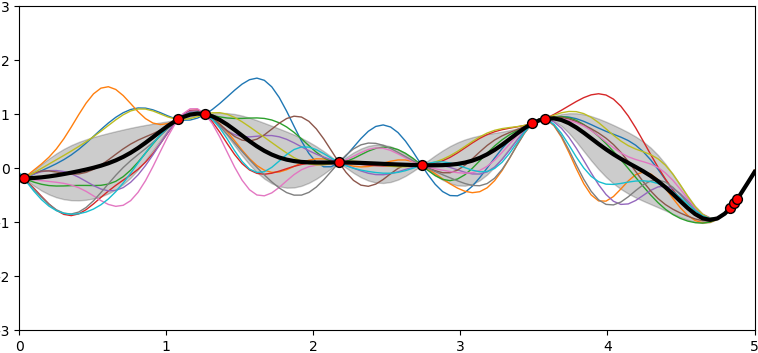
\includegraphics[width=0.45\textwidth]{RBF_posterior}
	\label{fig:RBF_posterior}}
	\caption[Prior and posterior of RBF kernel]
		{\hspace{-0.18cm}\footnotemark\ 
		Prior and posterior distributions of an RBF kernel with mean zero, resulted in a Gaussian process $\mathcal{GP}\left( 0 (\vec{x}), \Sigma(\vec{x}) \right)$.
		Each color line stands for a drawing (prediction) from the prior and posterior distributions, and the thicker black line shows the overall mean of the distributions.
		The red circles are the known data points on which the kernel was optimized to fit, and the gray areas mark the \SI{95}{\percent} confident intervals above and below the overall mean.
		The length scale parameter (in parentheses) determines the length of the \enquote{wiggles} of the functions}
	\label{fig:RBF_prior_posterior}
\end{figure}
\footnotetext{adapted from \url{https://scikit-learn.org/stable/_images/sphx_glr_plot_gpr_prior_posterior_001.png}}

As also motivated in \cref{subsec:limitations_of_did,subsec:temporal_analysis}, artificially splitting interactions into a fixed, pre-determined number of parts to measure accommodation results in a partial view on the process.
To avoid that, some interpolation method is required, with the goal of generating a more general behavior based on the observed productions.
This allows analysis on continuous series of values instead of point-by-point comparison, where the temporal gaps between data points might be greatly unbalanced.
One way of achieving that, using \ac{loess}, is shown in \cref{fig:hds_dds_time_pitch}.
A more evolve approach is presented here, where a speaker's vocal behavior is described as a distribution of functions that match the accumulated \textit{evidence} from the speaker's productions.
\todo{integrate these references}
\citet{Galvez2020unifiying}\\ % compare to the rather simplistic (and naive) approach taken here (based on TAMA) -- can refer to some of the specific methods there, specifically that they also use area under curve difference
\citet{Kousidis2008towards}\\ % original TAMA paper. read again, but seems like it's glorified moving average. say that my appraoch actually learns the curve of the speaker and doesn't just interpolate, which allows continuous predictions and more evolve description.
\citet{Kousidis2009monitoring}\\ % another TAMA paper, with an a bit more concrete example

Kriging (or \textit{\acl{gp} regression}) is an interpolation method that gives an optimally fitted and unbiased prediction of intermediate values.
\todo{references for a few fields where it is used?}
Since this method fits a function distribution over the data, it not only yields mathematically more likely values, but also provides a curve that describes the characteristics of the interpolated curved, as opposed to more naive methods like linear interpolation or smoothing spline.
Another advantage of this method is that it offers a \textit{distribution over functions} rather than specific values.
Therefore, an infinite number of suitable values can be drawn from one fitted kernel and their likelihood can be evaluated.
Such interpolation is illustrated in \cref{fig:RBF_posterior}, where each line represents a mean regression prediction drawn from the posterior distribution based on the given data points.

This method was applied on the dataset presented in \cref{sec:vacc}.
For simplicity, only the interactions in solo condition were used.
The functions prediction for a each speaker can be described by
%
\begin{equation}
	\label{eq:gp_function_prediction}
	f_*(\vec{x}) = \mathcal{GP}(\mu_{\vec{x}}, \Sigma_*),
\end{equation}
\eqname{Function predicted using a fitted Gaussian process}\noindent
%
where $\mu_{conv}$ is the mean feature value of a single speaker and $\Sigma_*$ is the fitted additive covariance function described in \cref{subsec:covariance_functions}.
It is important to note that the mean is not zeroed (as usually done in \ac{gp} regression) to maintain the original input values for the subsequent steps.
The kernel was initialized with the priors $C = 1$, $lengthscale = 1$, and no assumptions regarding noise level.
The search boundaries for the RBF and noise components were $1 < lengthscale < 100$ and $\num{1e-4} < \xi < 10$, respectively, with a maximum of six optimization iterations. % the initial one plus five allowed restarts (n_restarts_optimizer parameter in code)
% \xi is here the sign for noise
\todo[inline]{make sure these numbers are up to date}
\todo[inline]{write about how datapoints where selected from each turn to represent points of change}
With the fitted kernel, a continuous prediction can be made for each speaker over the entire conversation time span.
\Cref{fig:gp_vacc} shows an example of \ac{gp} predictions for one of the conversations. % 20171121A_Calendar_01 was used
%
\begin{figure}[t]
	\centering
	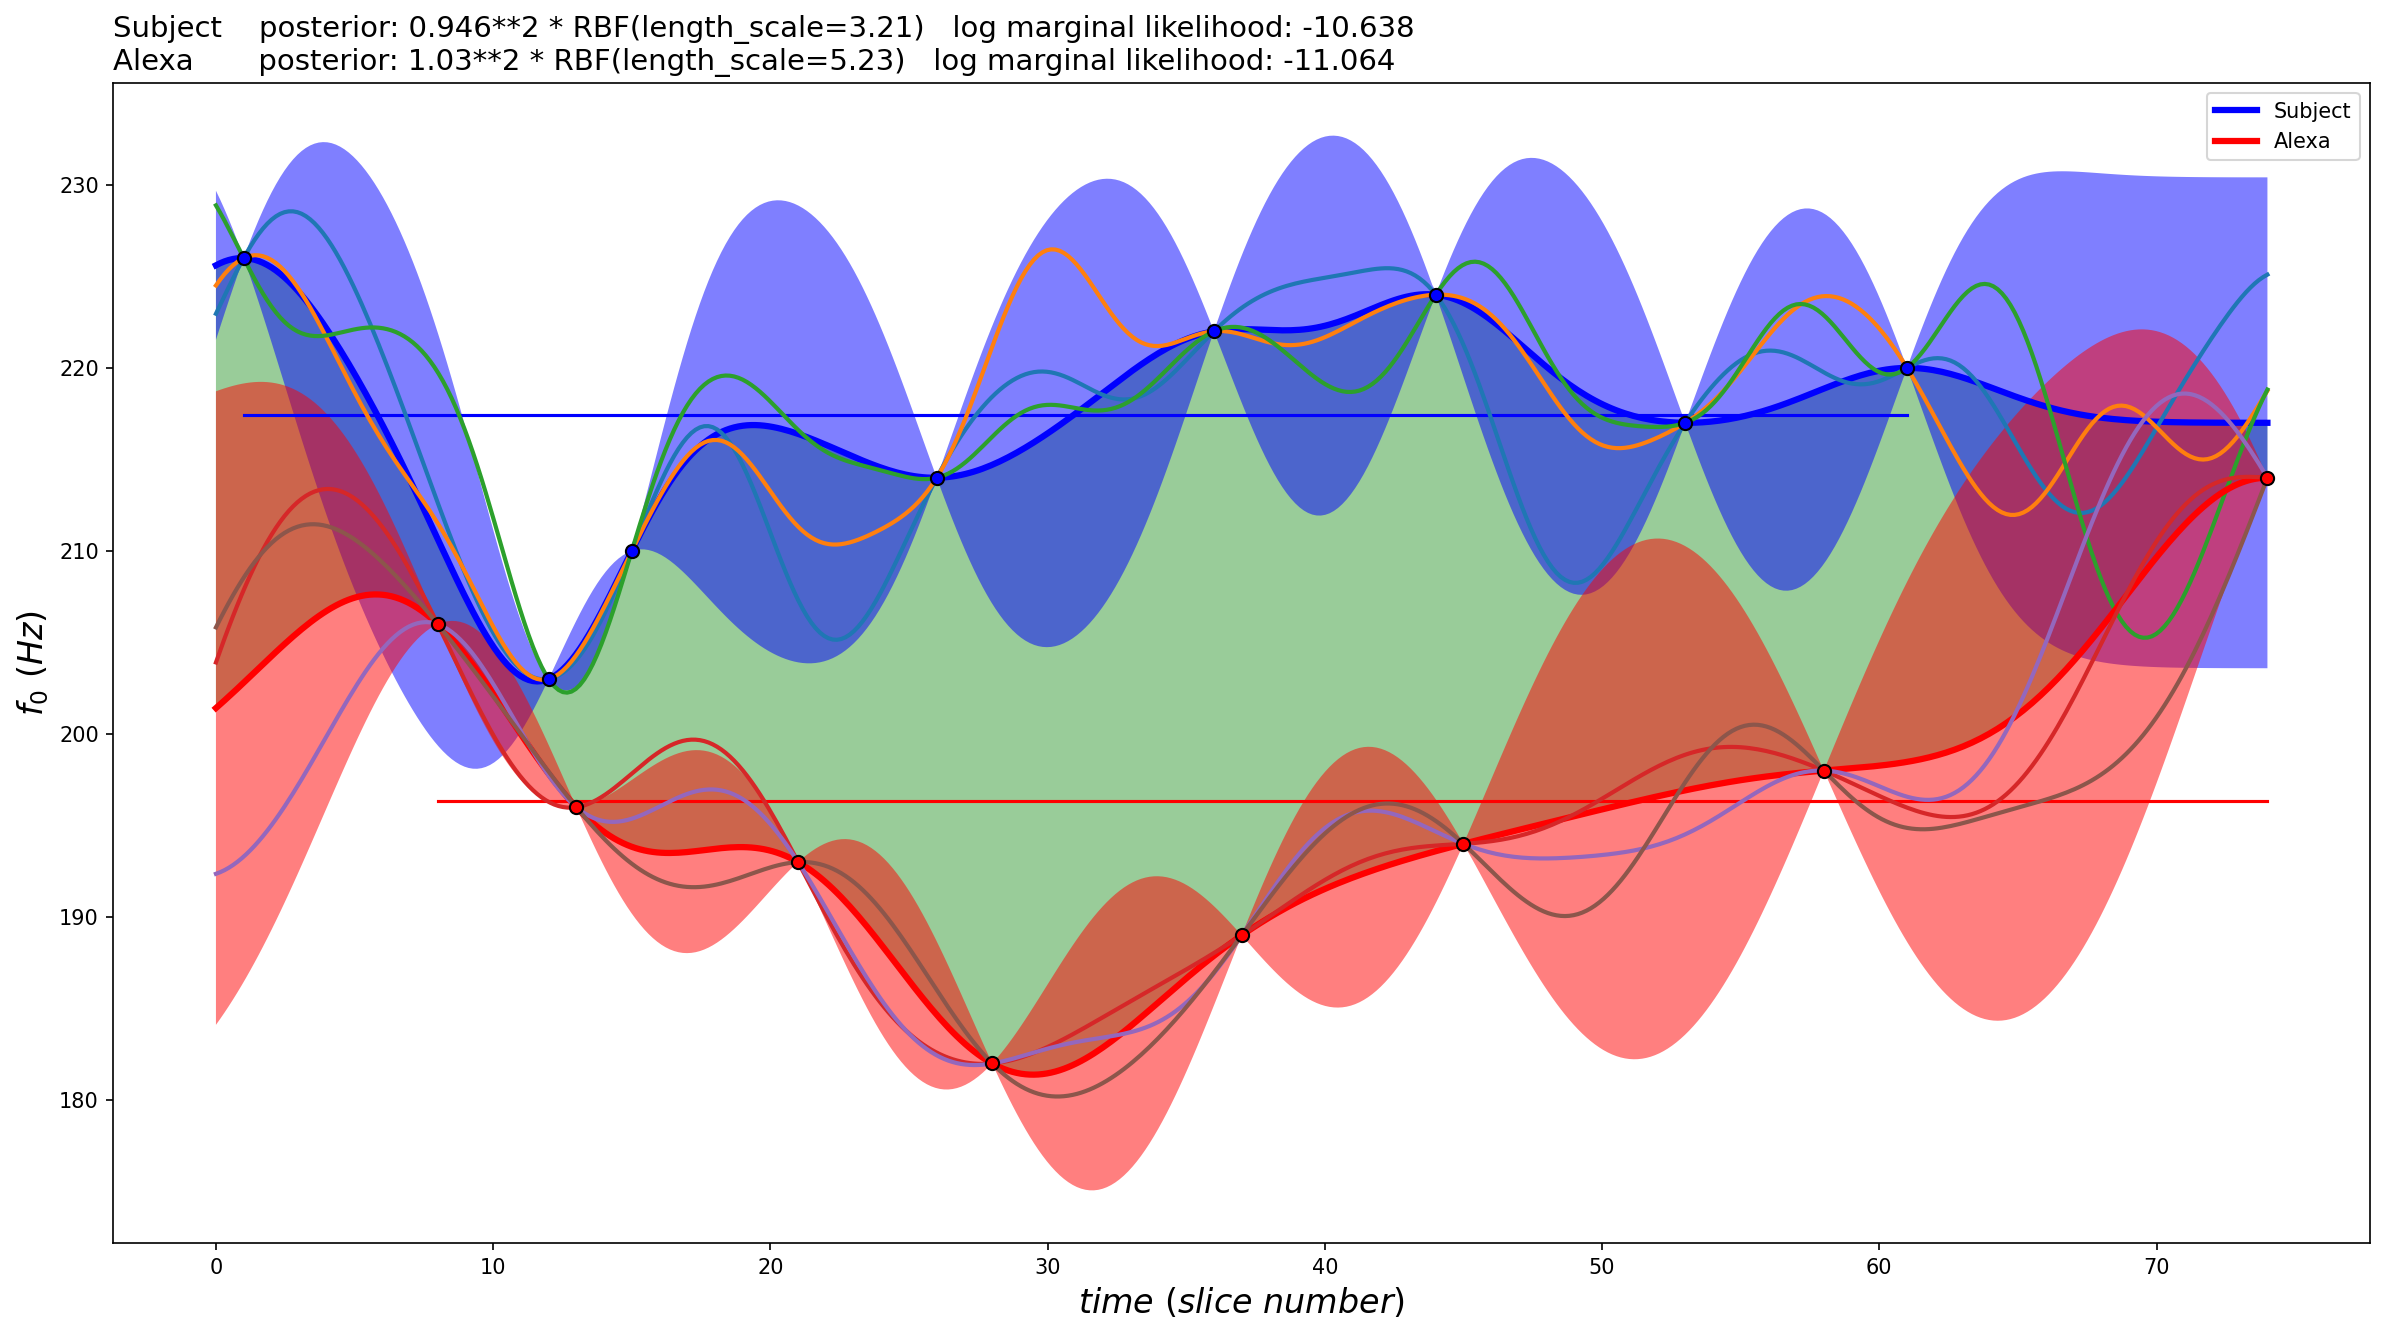
\includegraphics[width=\textwidth]{GP_VACC_with_draws}
	\caption[Gaussian process regression on conversation with Alexa]
		{Gaussian process regression for an interaction of a subject with Alexa.
		 The thick blue and red lines show the predictions' mean.
		 The additional lines around the means are randomly drawn functions from the fitted kernel representing potential variational output.
		 The colored areas around the means lines show the \SI{95}{\percent} confident interval for the distributions of the same color.
		 The straight horizontal lines indicate the overall mean of each speaker's productions.
		 The posterior parameters and the log marginal likelihoods of the fitted distributions are stated at the top.}
	\label{fig:gp_vacc}
\end{figure}

\section{Marking degrees of change}
\label{sec:measuring_changes}

Once a regression line is drawn for each speaker from their respective distributions, the differences between the speakers' productions can be measured.
Furthermore, due to the higher temporal resolution, more fine-grained degrees of change over time can be calculated as well.
The differences are calculated by the subtracting the trapped areas between the two regression lines (see \cref{fig:gp_vacc})
%
\begin{equation}
	f_{diff} \equiv\Delta\vec{x}_* =
	\int_{\vec{x}_i}^{\vec{x}_{j}}\mu_{f_*subject} -
	\int_{\vec{x}_i}^{\vec{x}_{j}}\mu_{f_*alexa}
\end{equation}
%
and the directional derivatives of the resulted delta line to measure the degree of change
%
\begin{equation}
	\nabla\Delta\vec{x}_*' = \frac{d}{dx}f_{diff}
\end{equation}
%
along the difference line.
\Cref{fig:diff_and_derivatives} demonstrates this on the same conversation from \cref{fig:gp_vacc} using the mean predictions of each speaker.
%
\begin{figure}[t]
	\centering
	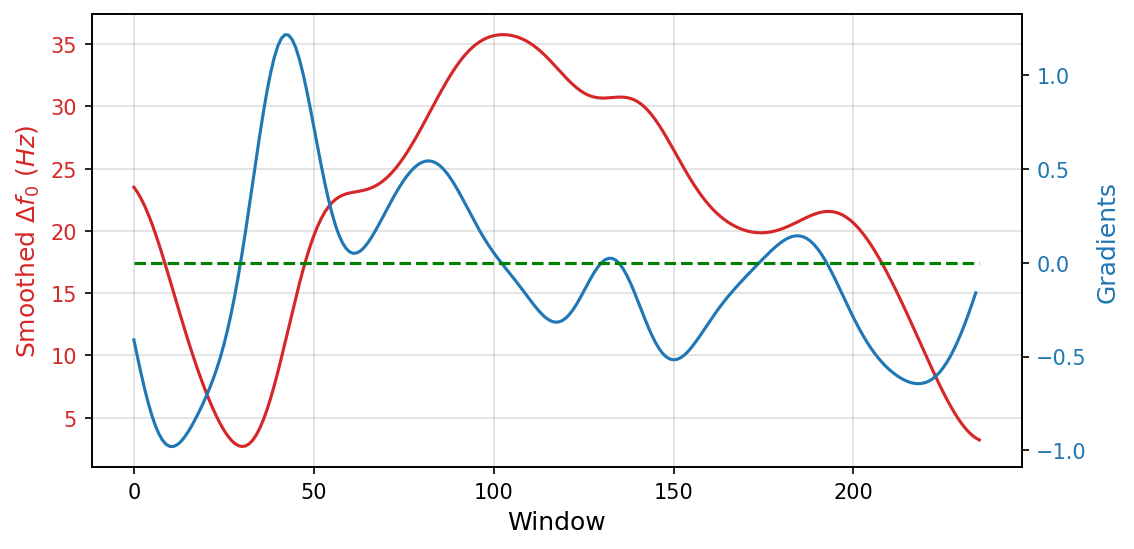
\includegraphics[width=\textwidth]{diff_and_derivatives}
	\caption[Continuous integral differences and derivatives in a \acl{hci}]
		{Continuous integral differences (red line) and their corresponding derivatives (blue line) of speakers' productions in a conversation.
		 The dashed green line shows the zero-gradient, , i.e., no change, threshold.}
	\label{fig:diff_and_derivatives}
\end{figure}
%
For building a generative model as described in \cref{sec:accommodation_as_a_lm,sec:clustering_and_incremental_generation}, the changes must be marked with pre-defined labels.
To that end, the derivative values were translated into a continuum of change ranging from \textit{divergence} to \textit{convergence}.
Based on this continuum, a discrete scale can be defined.
The more categories this discrete scale offers, the more specific the behavior descriptions can be.
\Cref{fig:cont_disc_scales} shows this process for a discrete scale of three categories: divergence, no (major) change, and convergence.
%
\begin{figure}[t]
	\centering
	\subfigure[Continuous scale]
		{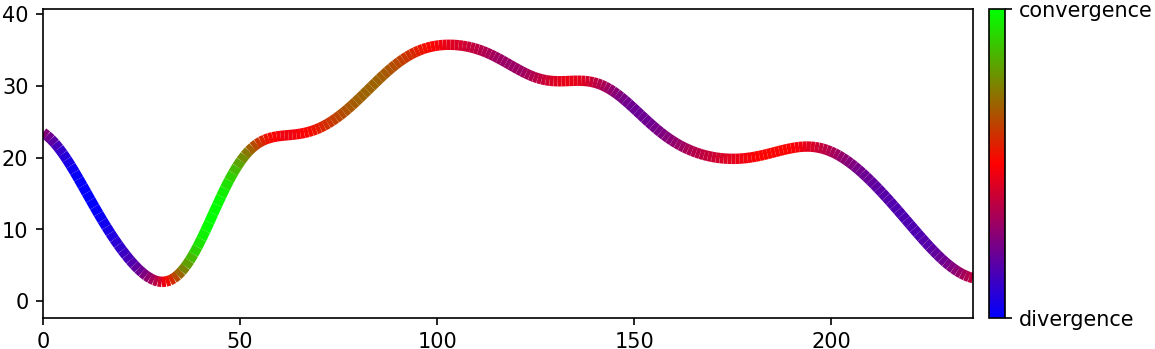
\includegraphics[width=0.47\textwidth]{cont_scale}
	\label{fig:continuous_scale}}
	\hfill
%	\vspace{-1cm}\hfill\hspace{-1cm}{\hbox{\LARGE $\Longrightarrow$}}\hfill
	\subfigure[Discrete scale]
		{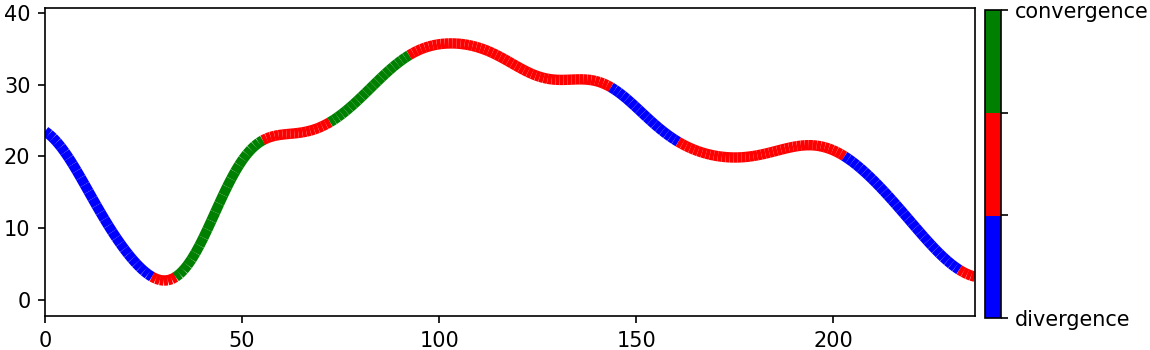
\includegraphics[width=0.47\textwidth]{discrete_scale}
	\label{fig:discrete_scale}}
	\caption[Continuous and discrete scales for labeling degrees of change]
		{Continuous and discrete color-coded scales for labeling degrees of change in a conversation.}
	\label{fig:cont_disc_scales}
\end{figure}
\todo[inline]{more details regarding how the discrete categories are defined}

\section{Accommodation as a language model} % Accommodation as an n-gram model
\label{sec:accommodation_as_a_lm}

In order to generate accommodation sequences, a model is needed, which can iteratively emits a label based on the seen labels history. 
Predictions of any model based on Markov decision process \citep{Bellman1957markovian} depend only on the current state of the conversation.
This neglects any temporal aspect of the conversation, which is a key component in spoken dialogue and accommodation \putref{cref to one or two places where this point is made}.
One way to overcome this is to extend the transition function of a Markov-based model, so that the previous $n$ states are somehow incorporated into the action $a$ of $P_a(s, s')$.
However, this violates the core idea of a Markov decision process and makes it cumbersome to use.
Therefore, an n-gram model is proposed here, which incorporates a portion of a sequence's history (or \emph{context}) into the decision making, without losing the Markov property.
The estimation of the element $e$ at position $i$ is therefore calculated by the probability term $P(e_i \mid e_{i-(n-1)},\ \ldots\ , e_{i-1})$.
N-gram models are traditionally used for describing sequences of some linguistic units, e.g., words in a language model \citep[e.g.,][]{Niesler1996variable}, and are used in applications like machine translation \citep{Marino2006ngram} and proteins identification \citep{Xu2015identification}.
The n-grams model here describes sequences of \emph{accommodation levels} across interactions.
These levels are represented by discretized values that are based on the degrees of change acquired in \cref{sec:measuring_changes}.
After computing the n-grams probabilities of the level, this model can be used for generating new sequences.
The resolution and variability of the model can be controlled by changing the n-grams' $n$ and the number of levels used to distinguish between the different accommodation levels.

\subsection{Dimensionality reduction and symbolic representation}
\label{subsec:dim_reduction_and_symbolic_rep}

The gradient time series extraction process described in \cref{sec:measuring_changes} (and see \cref{fig:diff_and_derivatives}) is greatly high dimensional, even for short interactions.
While this representation is useful for obtaining a fine-grained overview of the data, it is not practical for various analysis techniques that do not benefit (or are not designed to handle) such high dimensional data.
For instance, clustering algorithms, which need to iteratively compare between all points in a collection, scale better with lower dimensionality.
The dimensionality of the data in question here is reduced using \acf{paa} \citep{Keogh2001dimensionality}, which is a common dimensionality reduction technique for time series.
Each element $\vec{x}_i$ of the reduced vector is calculated by
%
\begin{equation}
	\label{eq:paa}
	\vec{x}_i = \frac{N}{n} \sum_{j=\frac{n}{N}(i-1)+1}^{i(\frac{n}{N})} S_j,
\end{equation}
\eqname{\Acl{paa} dimensionality reduction}\noindent
%
where $n$ is the dimensionality of the original times series, $1 \leq N \leq n$ is the dimensionality of the output vector, and $S_j$ is the $j$\textsuperscript{th} element of the original time series.
\Ac{paa} is suitable here, as the goal is to obtain vectors with fewer dimensions that still faithfully represent the data, and not, e.g., decompositions of the original data \citep[cf.\ method survey in][pp.\ 271-275]{Keogh2001dimensionality}.
As the goal here is to compare \emph{trends in change} within and across conversations rather than their absolute values, all gradient time series where z-normalized before applying the \ac{paa}.
Ultimately, \ac{paa} provides \textbf{continuous numeric values} that represent the overall shape of the original time series.
\todo{if eventually relevant, say that this normalization is reversed again when actual values are generated}
\Cref{fig:paa} illustrates \ac{paa} on the gradients of one of the interactions.

\begin{figure}[t]
	% 20171130A_Quiz_01 was used for these figures
	\centering
	\subfigure[\acs{paa} based on the original time seires.
			   The blue continuous line shows the original time series representing the mutual change gradients in a conversation, which was extracted as described in \cref{sec:measuring_changes}.
			   The organe circles show the \acs{paa} points created based on the continuous lines.
			   The dashed orange line is the linear interpolation between the \acs{paa} points.
			   Note that this lines is for illustration only and is not taken into account for any \acs{paa}-related analysis.]
		{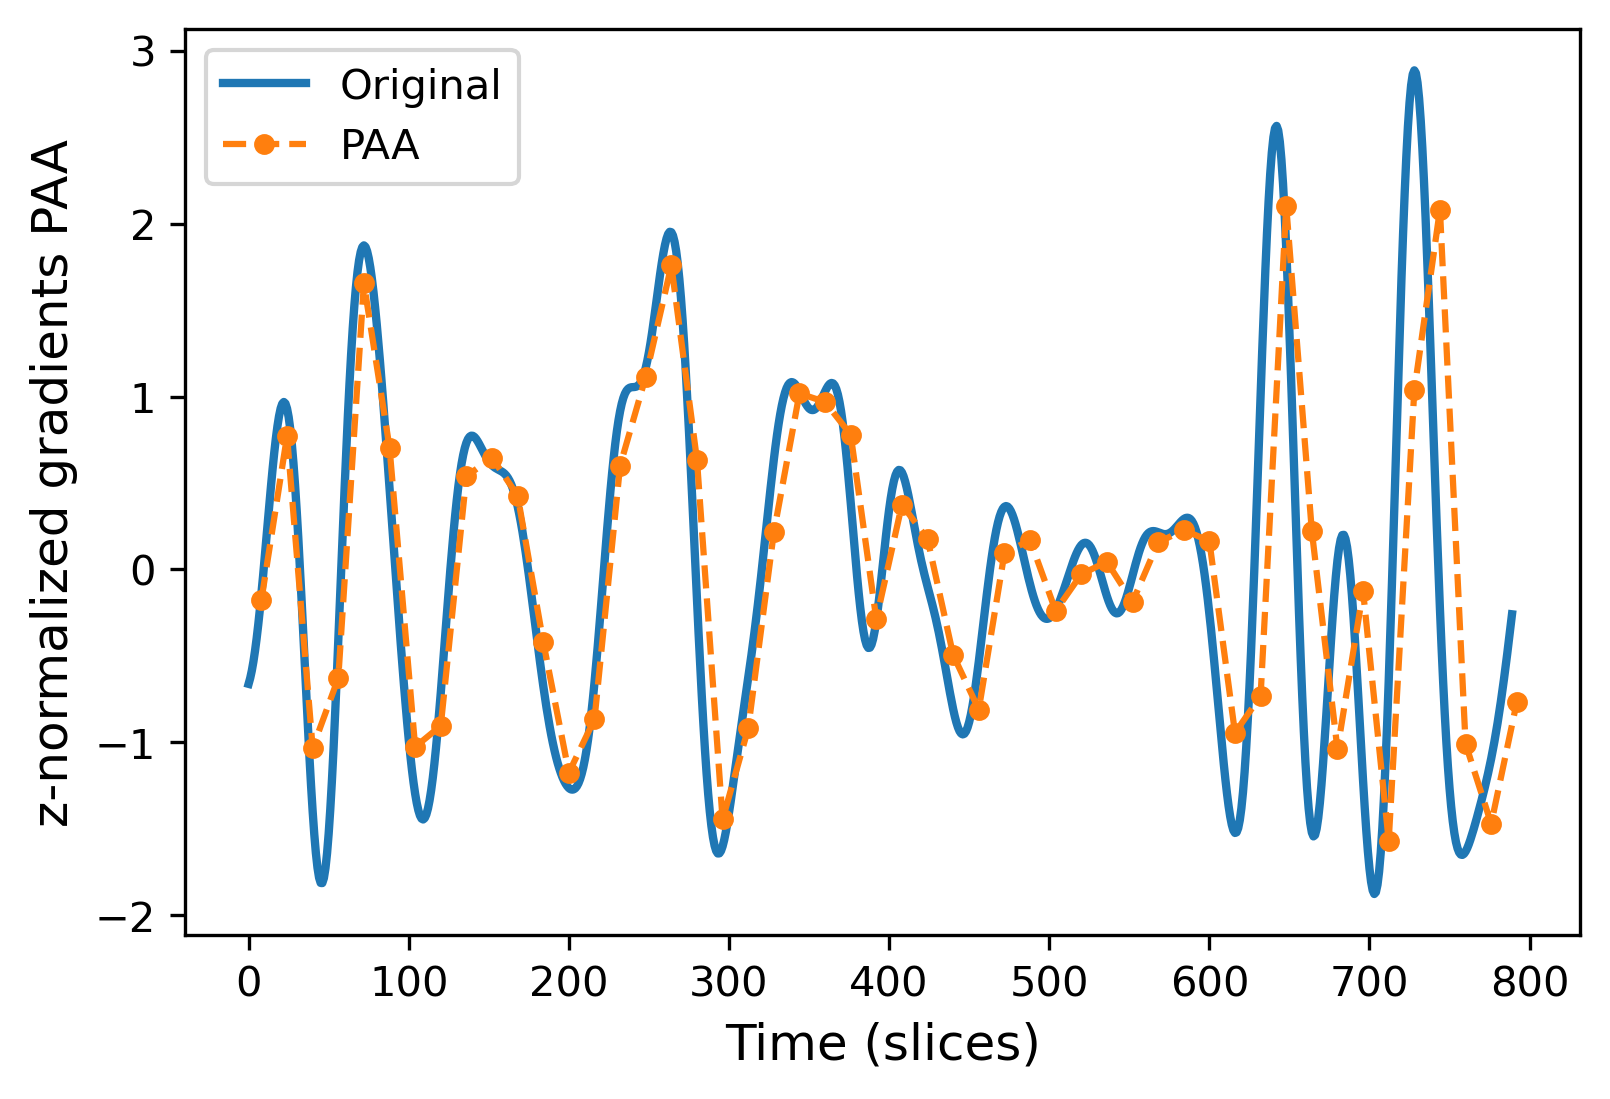
\includegraphics[width=0.47\textwidth]{PAA}
	\label{fig:paa}}
	\hfill
	\subfigure[\acs{sax} based on the \ac{paa} values.
			   The blue circles are the \acs{paa} points from \cref{fig:paa}.
			   The blue line visualizes the linearly interpolated trend of these points.
			   The horizontal green dashed lines show the margins of the five bins that split the points discrete categories derived from a normal distribution.
			   The organe labels (\enquote*{d+}, \enquote*{d}, \enquote*{n}, \enquote*{c}, and \enquote*{c+}) mark the classification of each point based on the bin it falls into.]
		{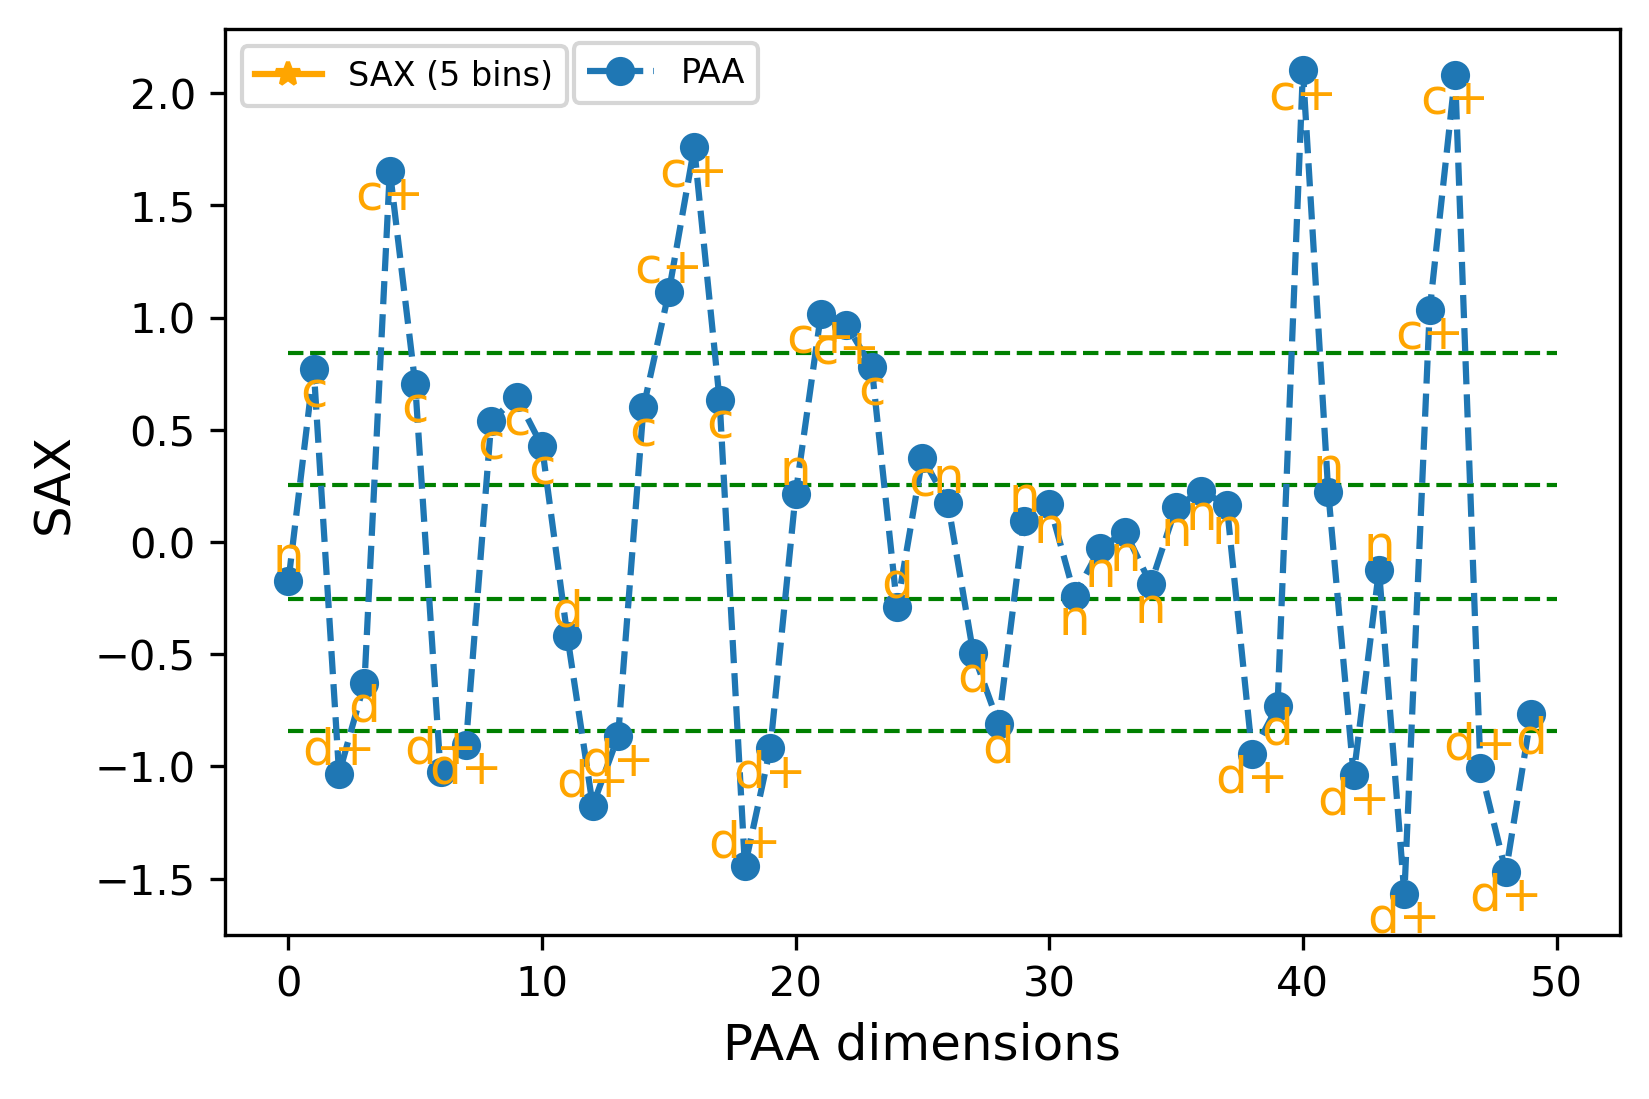
\includegraphics[width=0.47\textwidth]{SAX}
	\label{fig:sax}}
	\caption[\Acl{paa} and \acl{sax} for the time series representation of mutual change in a conversation]
		{\Ac{paa} and \ac{sax} for the time series representation of mutual change in a conversation.}
	\label{fig:paa_and_sax}
\end{figure}

\Ac{paa} is suitable for analyses of continuous numeric values.
However, discrete values are required for symbolic sequence-based processing, such as calculating probabilities of n-grams.
For converting the continuous \ac{paa} values, the \acf{sax} \citep{Lin2007experiencing} method was used.
\Ac{sax} assigns a string label to each of the pre-defined bins.
This is an advantage of \ac{sax}, as these labels provide a more meaningful and intuitive representation for humans.
As explained, e.g., by \citet{Apostolico2003monotony}, it is preferable to use a discretization technique that outputs a symbol set with equiprobability\footnote{It can be claimed that realistically equiprobability does not hold for the symbols in this kind of data.
While that may be true to some extent, neither the pre-processing nor the dimensionality reduction steps held any assumptions regarding the values in each \ac{paa} sequence.
Moreover, the data was z-normalized to avoid any bias stemming from specific numeric values.
For these reason, together with the fact that the participants were, in practice, free to speak in whatever way they wanted, equiprobability can be assumed in this analysis.
See \cref{subsec:word_extraction_and_seq_prob} for more information regarding the distribution of extracted symbol sequences}.
To that end, the \ac{sax} discretization was done using bins based on the normal distribution:
% this is defined by the method="normal" parameter in the SAX function (or `strategy` parameter internally)
\todo{can express the binning as a formula?}
Five categories (bins) are used here for categorizing degrees of change, labeled \enquote*{d+} for \emph{strong divergence}, \enquote*{d} for \emph{divergence}, \enquote*{n} for \emph{no (major) change}, \enquote*{c} for \emph{convergence}, and \enquote*{c+} for \emph{strong convergence}.
This number was found to adequately describe types of accommodation;
Three categories resulted in too unspecified sequences where all degrees of convergence or divergence are labeled similarly (as in \cref{fig:discrete_scale}), and seven or more categories did not add a substantial added value and often yielded in sparse sequences.
The motivation for choosing an odd number of categories is to have a \enquote{no-change} category.
However, an even number can be used as well, forcing each value to stand for either convergence or divergence while ignoring zero values.
Note that the term \emph{synchrony} is avoided here for describing steady distance between the speakers, per the definition introduced in \cref{subsec:variation_types}, which entails additional properties.
Ultimately, \ac{sax} provides \textbf{discrete textual labels}, which are a discretized version of the original time series.
\Cref{fig:sax} shows the \ac{sax} of mutual change time series based on the \ac{paa} points in \cref{fig:paa}.

\subsection{Sequence extraction and probability calculation}
\label{subsec:word_extraction_and_seq_prob}

After applying \ac{sax}, a sequence of accommodation labels was obtained for each corresponding interaction.
The count distribution of the labels was computed to examine their frequency.
As could be expected, the symbol $n$ (standing for no-change) had the highest frequency.
This frequency was about 2.5 times higher than the convergence and divergence labels $c$ and $d$, whose frequency, in turn, was roughly four times higher than the frequency of the strong convergence and strong divergence labels $c+$ and $d+$.
The same process was repeated for combinations of the labels as they appear in the \ac{sax} sequences.
The frequencies could be clearly separated into three groups:
Matching the single-label distribution, repeated $n$ labels were about three times more frequent than the second group, which consisted of most other combinations that included $n$.
Lastly, this group was followed by a longer tail of less frequent sequences, starting from counts three to four times lower, which included the rest of the symbol combinations.
Sequences with many repeated $c+$ or $d+$ labels (i.e., sustained convergence/divergence) always appeared at the end of the tail.
Increasingly smoother instances of the same overall distribution shape were found for all sequence lengths from two up to half the \ac{sax} sequence length (after which such frequencies become not as meaningful).
The percentage of covered n-grams of length $w$ found in the \ac{sax} sequences out of the $5^w$ theoretically possible combinations was exponentially lower the higher $w$ was.

\begin{table}[t]
	\centering
	\caption[Examples of probabilistically generated accommodation level label sequences]
		{Three examples of probabilistically generated accommodation level label sequences.
		 Each sequence consists of eight labels that were generated based on the initial context of the padding symbol $p$.
		 The first line of each example shows the generated symbols as introduced in \cref{subsec:dim_reduction_and_symbolic_rep} and their average variability (value between 0 and 1, higher number means more variability.).
		 The second line lists the scores (probabilities) of each corresponding generated label given the context seen up to that point and the overall probability of generating this entire sequence.
		 The third line lists the perplexity of the trigram ending with the corresponding generated label given the context at the time of the generation.
		 Note that the first two padding labels do not have score values, as they are given as the initial context.
		 Similarly, perplexity can only be calculated once the sequence is longer than the one trigram.}
		 % variability was calculated as the average "deviation", where c and d have value of 0.5, c+ and d+ value of 1, and n value of 0. for Example (c + c+ + n + n + d+ + c + n + n) / 8 = 0.375
	\label{tab:generated_symbol_sequences}
	\begin{tabularx}{\linewidth}{*{10}{c}l@{\hskip 0.1cm}l}
		\toprule
		p    & p    & n    & n    & n    & c    & n    & d    & d    & c    & variability: & \num{0.187}  \\
		---  & ---  & 0.44 & 0.46 & 0.55 & 0.18 & 0.32 & 0.29 & 0.25 & 0.35 & probability: & \num{1.63e-4}\\
		---  & ---  & ---  & 2.22 & 1.99 & 3.16 & 4.16 & 3.27 & 3.67 & 3.35 & perplexity: & \num{3.11}   \\[0.4cm]
		
		p    & p    & n    & d    & d    & c    & c+   & d+   & d+   & c+   & variability: & \num{0.687}  \\
		---  & ---  & 0.44 & 0.17 & 0.25 & 0.35 & 0.13 & 0.25 & 0.34 & 0.19 & probability: & \num{1.37e-5}\\
		---  & ---  & ---  & 3.67 & 4.88 & 3.35 & 4.69 & 5.62 & 3.46 & 3.96 & perplexity: & \num{4.23}   \\[0.4cm]
		
		p    & p    & c    & c+   & n    & n    & d+    & c     & n    & n    & variability: & \num{0.375}  \\
		---  & ---  & 0.30 & 0.25 & 0.25 & 0.16 & 00.04 & 00.20 & 0.22 & 0.41 & probability: & \num{2.16e-6}\\
		---  & ---  & ---  & 3.67 & 4.03 & 5.02 & 12.72 & 11.51 & 4.77 & 3.30 & perplexity: & \num{6.43}   \\
		\bottomrule
	\end{tabularx}
\end{table}

N-grams of $n = 3$, i.e., trigrams, were used here for computing the probabilities.
The size of the n-gram determines the amount of previously acquired evidence that can be use to calculate a subsequent value.
This fulfills the same role as the \emph{pool size} parameter of the computational model (see \cref{sec:parameters}).
In both cases, the goal is to account for the temporal evolution of the conversation for deciding on its continuation.
To account for conversation-initial sequences, the beginning of each symbol sequence was padded.
The end of the sequence was not padded, since, unlike a traditional language model, the generative model here lets the user decide on the end of the interaction (see \cref{sec:clustering_and_incremental_generation}).
This summed up to a collection of \num{2700} trigrams, which comprised 143 out of the $5^3$ level combinations~1~$\times$~5~two-padding combinations~+~5~$\times$~5~one-padding combinations~$= 155$~possible symbol combinations (\SI{92}{\percent}).
% 2700 is 54 solo interactions times 50 trigrams for each: the size of SAX used was 50, which gives 48 trigrams. with the 3 trigrams added from padding, it's 50. 50 times 54 = 2700
This shows a great variety in conversation dynamics.
% however, since not all possible combinations are used for training, unseen trigrams can still be seen during generation. we set the vocab to be all possible combinations (plus all initial padded trigrams)
% smoothing??
% probabilities for OOV trigrams?
Based on this n-grams model, sequences of symbols, representing accommodation levels in a conversation, can be probabilistically generated.
For example, the next accommodation level $l$ after two convergence labels is taken from the probability distribution $p(l \mid c,\ c)$.
\Cref{tab:generated_symbol_sequences} shows examples of such probabilistically generated sequences for the eight first accommodation labels of a conversation.
It is worth noticing that the third sequence in the table has lower variability than the second sequence, although its overall probability is lower and its mean perplexity is higher.
That means that, based on this model, interactions with lower variability are not necessarily more likely.
On the other hand, since in most context the probability of label $n$ is relatively high, sequences with many $n$ labels are more likely to appear, on average.

\section{Clustering and incremental variational generation}
\label{sec:clustering_and_incremental_generation}

After defining a unified representation of the mutual changes in interactions over time in \cref{subsec:dim_reduction_and_symbolic_rep}, the question arises whether clusters in these representation can be found to detect general similarities in behavioral patterns.
Two clustering methods are, namely \ac{knn} and hierarchical linkage, each offering a different angle and insights.
The former method is a top-down approach with a pre-defined number of clusters, which offer a more general view on the patterns, and latter a bottom-up approach with no prior assumptions, where more speaker-specific differences can be measured.
It cannot be expected to find completely distinct pattern for each speaker.
However, some separable clusters and general tendencies are expected to emerge, both when inspecting individual speakers and at the collection as a whole.

\todo[inline]{if it's not too much work, see how many subject end up having both their interactions in the same cluster}

\todo[inline]{try look into the clusters to see if they can be defined/described somehow (this is where Alexander's visualization can be used)}

\begin{figure}[t]
	\centering
	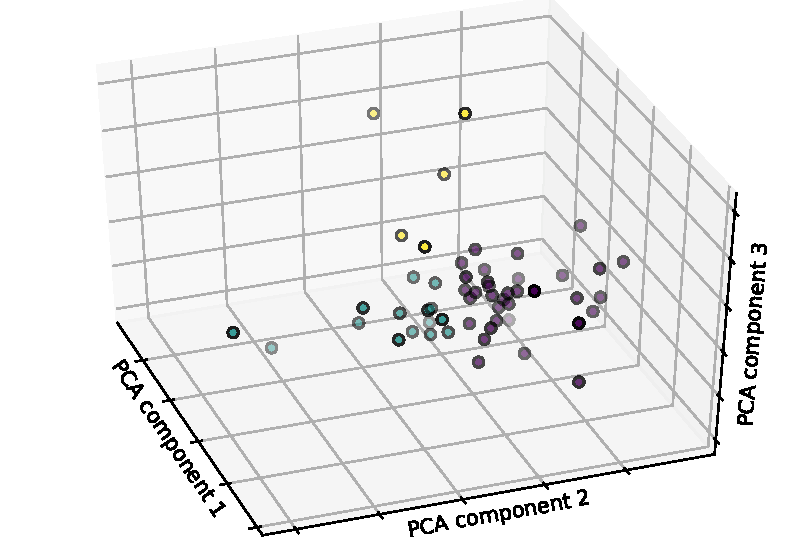
\includegraphics[width=\textwidth]{3d_clustering}
	\caption[3D \ac{knn} clustering of mutual changes \ac{pca} components]
		{\ac{knn} clustering of the first three \ac{pca} components of the interactions' \ac{paa} sequences.
		 Each circle represents one sequence in the three-dimensional space.
		 A circle's color indicates the cluster to which the datapoint belongs.}
		 % elevation is 40 azimuth is 160
	\label{fig:knn_clustering}
\end{figure}

Since the \ac{paa} representations created in \cref{subsec:dim_reduction_and_symbolic_rep} can be arbitrarily long and high dimensional, they are reduced here to their $n$ first \ac{pca} components for the purposes of visualizing their clustering.
The k-nearest neighbors algorithm was used for clustering.
the process was performed for 2, 3, and 5 clusters using the 2 or 3 first \ac{pca}, with the combination of 3 clusters and 3 components performing the best on average.
% on average since kNN is not deterministic and was run multiple times
The result is shown in \cref{fig:knn_clustering}.

\todo{need references for PCA and kNN?}

\begin{landscape}
	\begin{figure}[t]
		\centering
		\hspace*{-4cm}
		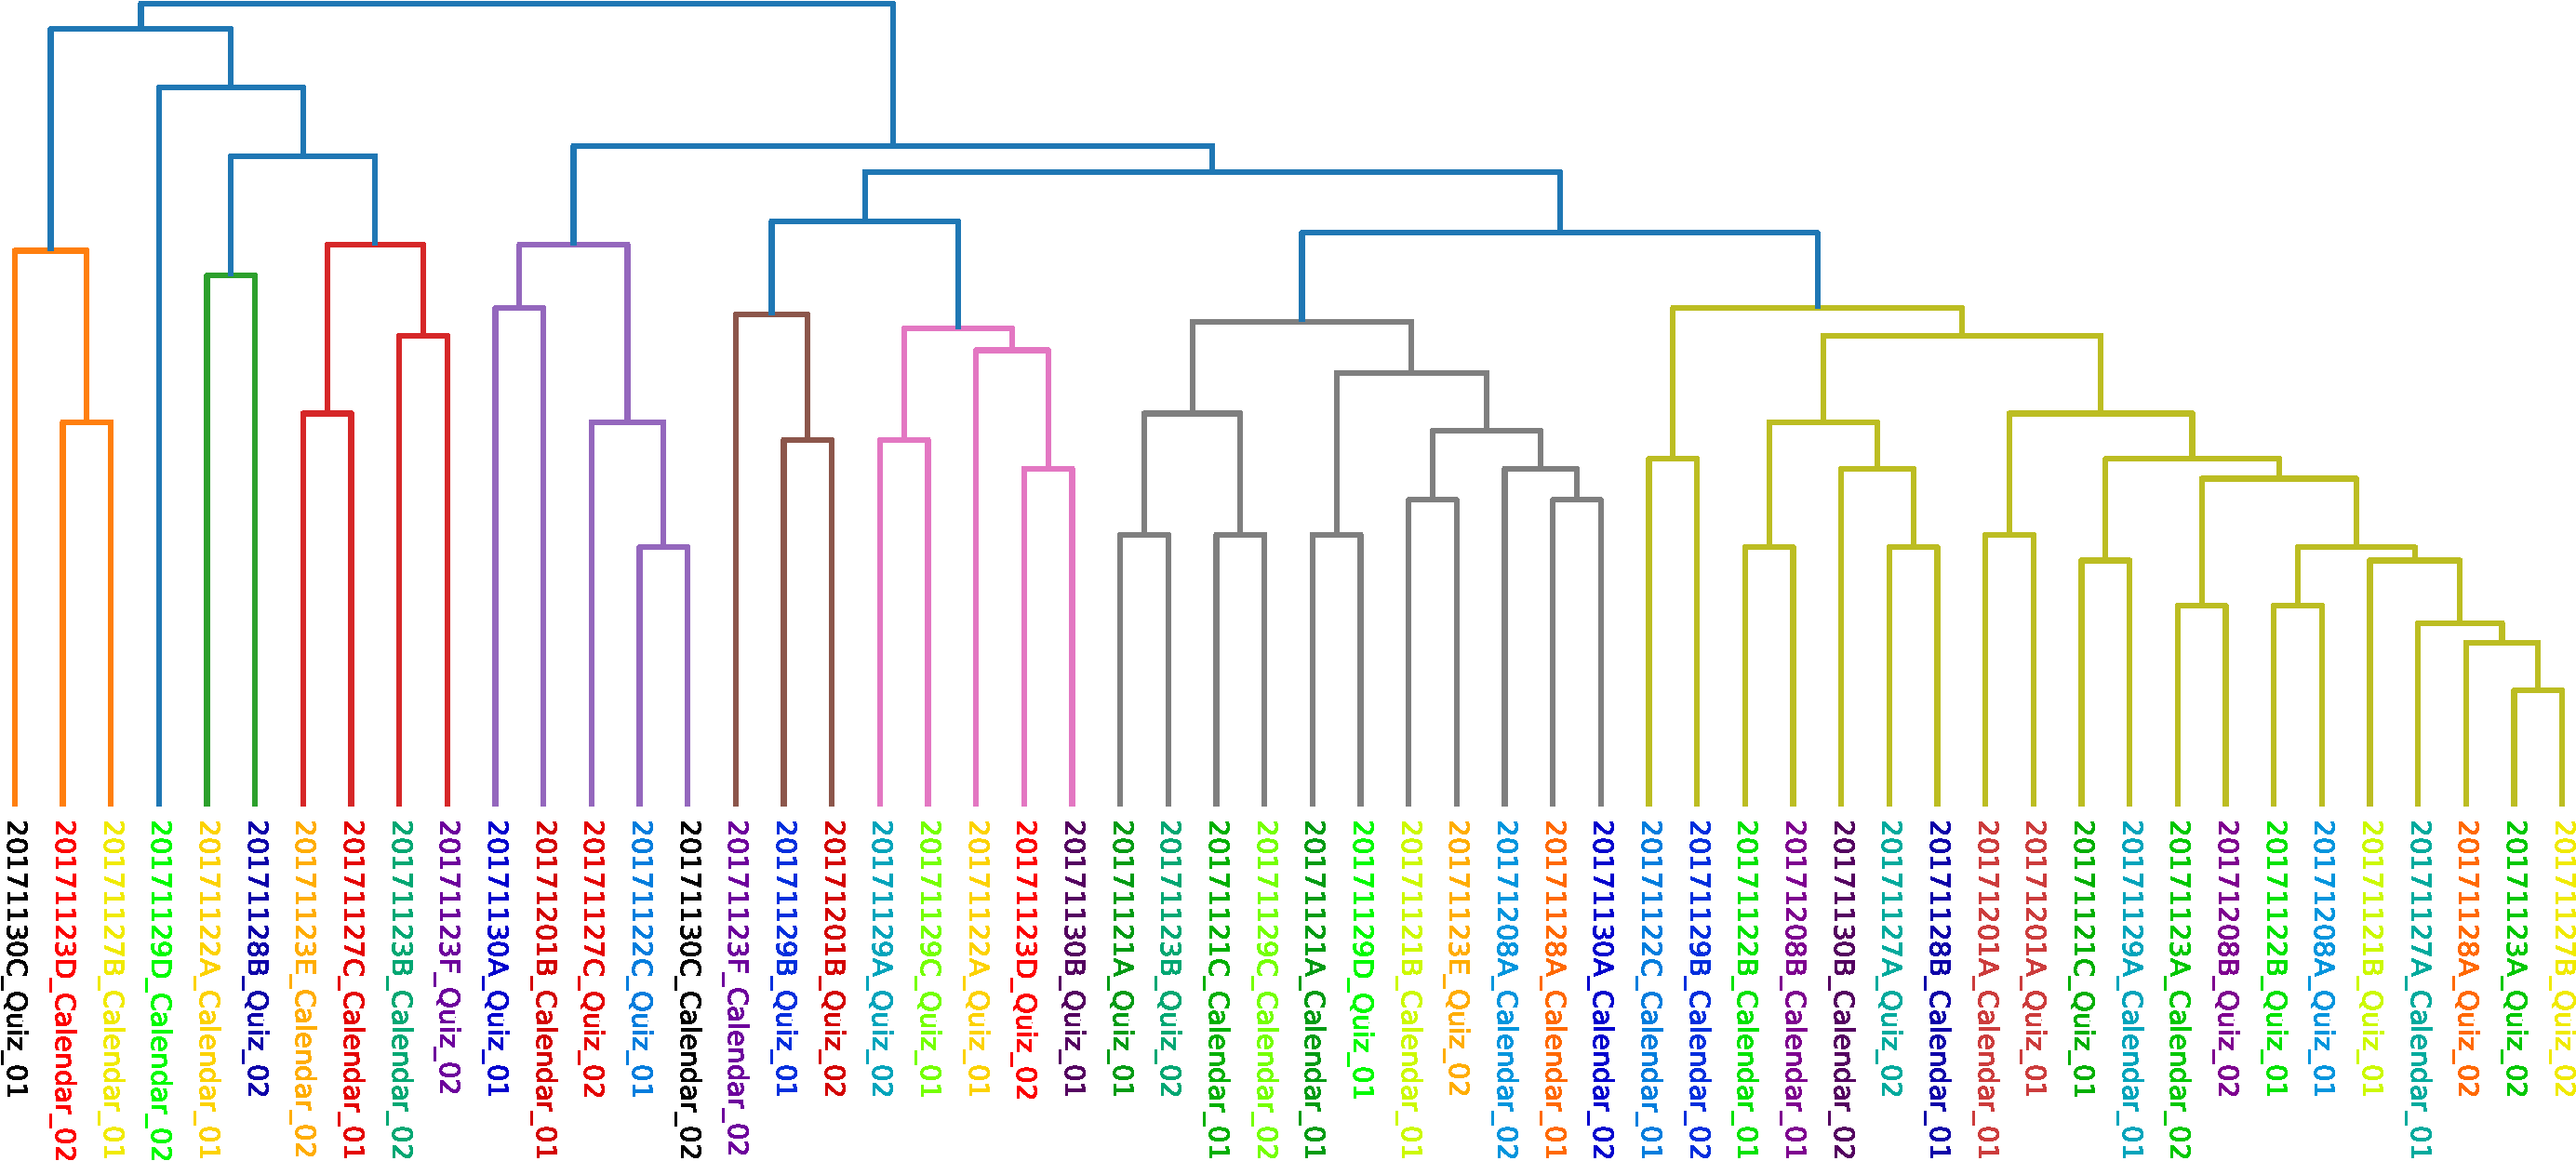
\includegraphics[width=1.7\textwidth]{paa_dist_dendrogram}
		\caption[Dendrogram of time series representation of interactions distances]
			{Dendrogram of the time series \ac{paa} representations of the solo condition interactions based on complete-link distances.
			 Each cluster is represented by a different color of lines.
			 Blue lines connect pairs of clusters that are most similar to each other, and similarly pairs of the closest subsequent sub-cluster and eventually leaves are connect directly to each other.
			 Each leaf represent the interaction indicated by its label.
			 Labels of the same color mark interaction with the same subject (two interactions per subject).
			 The leaf and cluster colors are \emph{not} related.
			 The leaves are order horizontally by their distance from left to right, so that the leaves of interactions that are more similar to each other (both inter- and within-cluster) are positioned closer.
			 For example, the two interactions of subject \emph{20171201A} (12\textsuperscript{th} and 13\textsuperscript{th} leaves from the right) are the closet to each, as they are positioned together and within the same smaller sub-cluster.}
		\label{fig:paa_dist_dendrogram}
	\end{figure}
\end{landscape}

While top-down clustering can uncover general grouping of elements, bottom-up hierarchical clustering can reveal structural relations between them and measure their degrees of similarity.
With numeric values assign to the degrees of changes along an interaction via the the \ac{paa} representations created in \cref{subsec:dim_reduction_and_symbolic_rep}, the distances between the 54 interactions can be measured and compared.
The calculation was done using \emph{complete link} (a.k.a.\ farthest point algorithm) agglomeration technique.
This kind of linkage is supported by the assumption that there are more general behavior patterns beyond the individual differences, as it searches the most dissimilar (and hence principally all) interactions in neighboring clusters and not only the closest one.
This method also allows using the entire \ac{paa} sequences.
\Cref{fig:paa_dist_dendrogram} shows the bottom-up distance clustering based on this linkage. 
Although, unsurprisingly, no definite order emerges, some general trends can be seen regarding the similarity between interactions of the same subject.
As the leaves are ordered horizontally based on their overall similarity, the distances between their positions be utilized to determine each subject's behavior consistency.
The average distance of the population is 16.5, far from the maximal possible average of 27.
% This is the maximal possible average, since this is when each interaction is half of the population away from its pair.
% With the largest possible distance between two leaves being 53, the space can be divided into three bins of 18 (rounded up).
Dividing the space into three equal bins of \enquote{short}, \enquote{medium}, and \enquote{long} distances shows that 16, 10, and 1 interaction(s) fall into these bins, respectively.
Moreover, this distribution has median of 16 and its second tertiles located at 19, far from the \enquote{long distance} bin.
Such skewness in the distribution indicates that interactions of the same speaker tend to be relatively similar in terms of accommodation trends, regardless of any other factor (interaction length, task, order, and other factors used in \cref{chap:speech_variations_in_hhci}).
Notably, the two interactions of one participant, 20171201A, even have the minimal possible distance of 1 between them (12\textsuperscript{th} and 13\textsuperscript{th} leaves in \cref{fig:paa_dist_dendrogram}) and they are located together in the smallest sub-cluster.

\todo[inline]{if the generation based on cluster really works decently, refer to this section when describing variational vocal behavior as one of the levels for accommodative SDS}

\todo[inline]{if it's not too much work, calculate how many subjects are in the same-color cluster}.